\documentclass[xcolor=table]{beamer}

\usepackage{lscape, amsmath, amsfonts, amssymb, setspace, theorem, wrapfig, graphicx, float, multirow, subfig, color, rotating, multicol, datetime, natbib, venndiagram, pstricks, xkeyval, tikz, etoolbox, url, hyperref, nth}

\usepackage[T1]{fontenc}
\usepackage[latin1]{inputenc}
\usepackage[english]{babel}

\title{GV217 - Conflict Analysis}
\subtitle{University of Essex - Department of Government}
\date{Week 17 -- 24 January, 2020}				% or you can specify a date, just write it down instead of "\today"
\author{Lorenzo Crippa} 

\usetheme[progressbar=frametitle]{metropolis}
\usecolortheme{seahorse}						% try others: wolverine; crane...

\begin{document}
\frame{
\titlepage
}

\frame{
\frametitle{Recap of last seminar}
\textbf{State-based armed conflict}:
\begin{itemize}
\item Intrastate (within)
	\begin{itemize}
	\item[--] With foreign involvement (internationalized)
	\end{itemize}
\item Interstate (between)
	\begin{itemize}
	\item[--] Extrastate
	\end{itemize}
\item At least one actor is the government
\item Incompatibility
	\begin{itemize}
	\item[--] Government
	\item[--] Territory
	\end{itemize}
\item Use of armed force between the TWO parties \ldots
\item \ldots at least 25 battle-related deaths in a year
\end{itemize}

\textbf{Non-state violence}: violent conflict between non-state actors

\textbf{One-sided violence}: targeted killing of civilians (by the state or non-state actors)
}

\frame{
\frametitle{Recap of Thursday's lecture: How safe is the world today?}
\begin{itemize}
\item Pinker's argument: decline in violence. Why? \pause
	\begin{enumerate}
	\item The state as a peace keeper
	\item Trade and economic interdependence
	\item Feminisation and female political participation
	\item Cosmopolitanism
	\item Education, norms, spread of reason
	\end{enumerate} \pause
\item Criticism: has there been such a decline, though? \pause
	\begin{enumerate}
	\item Western-centric argument (data, authors)
	\item Many wars (WWI, WWII, \nth{18} and \nth{19} century) waged by states, often for commerce
	\item Cultural and material/institutional factors are entangled
	\item Change time scale or statistics: Data tell different stories
	\item What about geographical distribution of conflict?
	\end{enumerate}
\end{itemize}
}

\frame{
\frametitle{A few examples of recent conflicts in the news}
\begin{itemize}
\item Conflict in Darfur (Sudan)
\item Rohingya in Myanmar
\item Burundi conflict (Hutu and Tutsi)
\item Nagorno-Karabakh conflict (Armenia-Azerbaijan) \pause
\end{itemize}

Try to classify them!
}

\frame{
\frametitle{First assignment}
Fist assignment due in week 18
\begin{enumerate}
\item List the UCDP recorded conflicts in \textbf{2018}
\item Describe the conflicts: What patterns do you see among them?
	\begin{itemize}
	\item Readings and definitions of last week
	\item UCDP data discussed this week
	\end{itemize}
\end{enumerate}
Resources from Uppsala Conflict Data Program (UCDP):

UCDP \textbf{definitions}: \href{https://www.pcr.uu.se/research/ucdp/definitions/}{click here} \\ UCDP \textbf{data}: \href{https://ucdp.uu.se/exploratory}{click here}
}


\frame{
\frametitle{UCDP (Uppsala Conflict Data program}
Today we'll work on UCDP data. \pause

Go to \url{https://ucdp.uu.se/downloads/} \\
The data we need are under the label ``UCDP/PRIO Armed Conflict Dataset version 19.1'' \pause
\begin{enumerate}
\item Download the Codebook \\ \pause
Key variables: type of conflict, incompatibility \\ \pause
Actors: side A \emph{vs.} side B, intensity level \\ \pause
Missing data: -99 \\ \pause
Unit of analysis: conflict-year \pause
\item Download the Data and open in Microsoft Excel
\end{enumerate}
}

\frame{
\frametitle{Questions to consider}
\begin{itemize}
\item How many conflicts were there in 2018? \pause
\item How many are state-based? \pause
\item Can you identify some patterns? \pause
	\begin{itemize}
	\item[--] Is there an actor that is active in several conflicts? 
	\item[--] What type of conflict is most common? Intra or inter-state?
	\item[--] In which region do most conflicts take place?
	\item[--] What are most conflicts about?
	\item[--] How many of the conflicts can be classified as war?
	\item[--] How many have been internationalized?
	\end{itemize}
\end{itemize}
}

\frame{
\frametitle{Exercise}
Exercise of today. Get in groups of two:
\begin{enumerate}
\item List the UCDP recorded conflicts in \textbf{2016}
\item Describe the conflicts:
	\begin{itemize}
	\item How many conflicts in 2016?
	\item How many are state-based?
	\item Can you identify some patterns?
		\begin{itemize}
		\item[--] Is there an actor that is active in several conflicts? 
		\item[--] What type of conflict is most common? Intra or inter-state?
		\item[--] In which region do most conflicts take place?
		\item[--] What are most conflicts about?
		\item[--] How many of the conflicts can be classified as war?
		\item[--] How many have been internationalized?
		\end{itemize}
	\end{itemize}
\item Present your results (bullet points). Discuss with the class
\end{enumerate}
}

\frame{
\frametitle{How many conflicts? What actors?}
How many conflicts in 2016? How many are state-based? \pause \\ \textbf{53 conflicts} \pause

Is there an actor that is active in several conflicts? \pause \\ The IS is active in 15 conflicts, most active non-state actor. \\ \pause Governments of India and Pakistan are active in 4 conflicts each, most active state-actors. 
}

\frame{
\frametitle{What type of conflict is most common?}
\begin{figure}
\centering
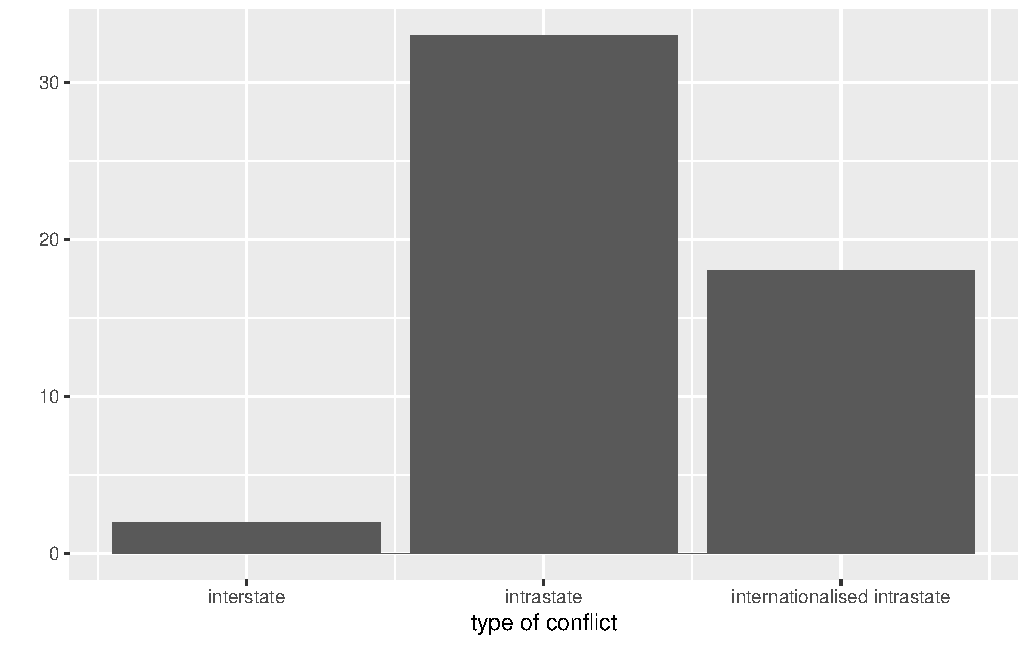
\includegraphics[width=110mm]{pictures/week_17_1.pdf}
\end{figure}
}

\frame{
\frametitle{In which region do most conflicts take place?}
\begin{figure}
\centering
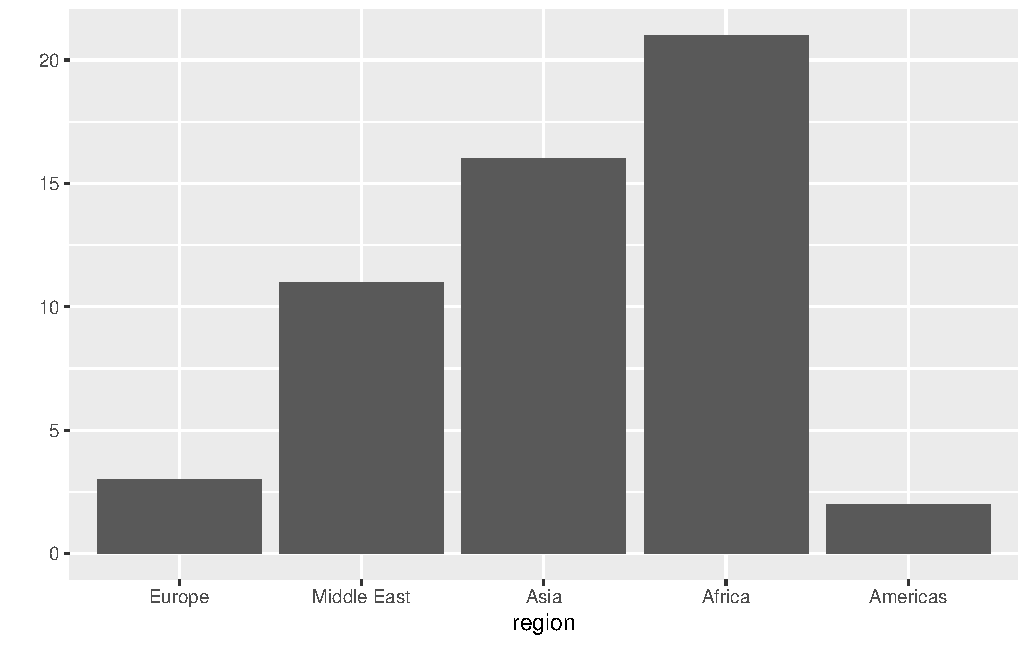
\includegraphics[width=110mm]{pictures/week_17_2.pdf}
\end{figure}
}

\frame{
\frametitle{What are most conflicts about?}
\begin{figure}
\centering
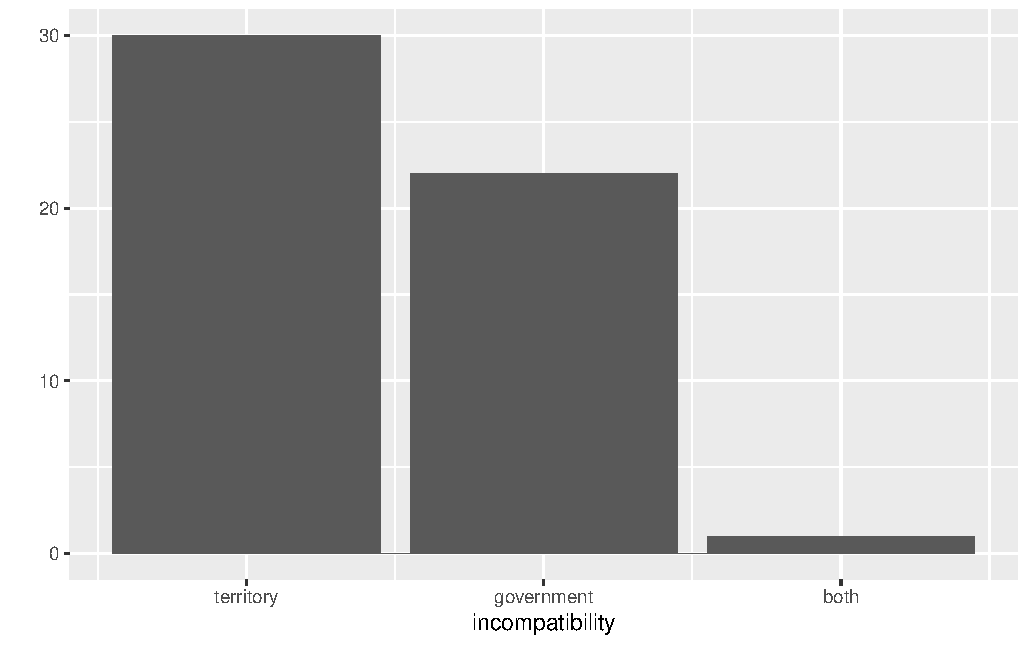
\includegraphics[width=110mm]{pictures/week_17_3.pdf}
\end{figure}
}

\frame{
\frametitle{How many of the conflicts can be classified as war?}
\begin{figure}
\centering
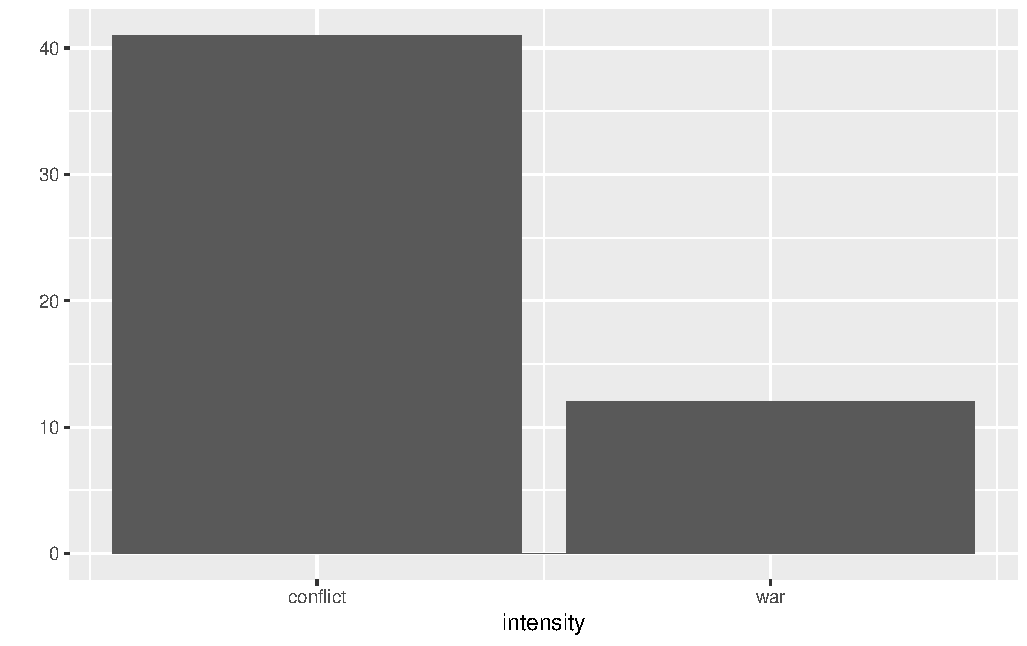
\includegraphics[width=110mm]{pictures/week_17_4.pdf}
\end{figure}
}

\frame{
\frametitle{Further resources to study conflicts}
\begin{itemize}
\item Research Institutions: e.g., UCDP, ACLED
\item Think Tanks: e.g., Crisis Group, Chatham House, Carnegie, Council on Foreign Relations
\item NGOs: e.g., Amnesty International, International Red Cross
\item International news outlets: e.g., BBC, NYT, Aljazeera
\end{itemize}

Include as many resources as possible to prevent bias! 
}

%\frame{
%\frametitle{A few questions to conclude}
%\begin{itemize}
%\item Do you think we live in a less violent world? In absolute or relative terms? Why? \pause
%\item Are people inherently prone to use violence? \pause
%\item What is the role of the international system and power balance? \pause
%\item What role will new trends in climate change, technology and alike play in the future? \pause
%\item Can ``institutions'' be our savior? Governments, IOs etc. 
%\end{itemize}
%}

\frame{
\frametitle{Conclusion}
\begin{center}
All clear? More questions? \\
See you next week!
\end{center}
}


\end{document}
